\section{Présentation de la méthode PINN}

\subsection{Introduction et état de l'art}

L'utilisation des techniques d'apprentissage machine aux domaines dits "classiques" comme la mécanique n'est pas nouveau. De nombreux travaux de recherche ont été menés jusqu'aux applications industrielles pour des problèmes d'aide à l'optimisation, de contrôle, de pré-développement de pièces ou de modèles réduits dont on pourra se faire une idée avec la synthèse de \cite{bruntonMachineLearningFluid2019a}. Néanmoins l'approche privilégiée a été celle des données, \textit{data-driven} comme on le trouve dans la littérature. Cela signifie que les réseaux de neurones encodent les mécanismes physiques (dans le meilleur des cas) uniquement à partir d'un certain nombre de données préparées au préalable. Par exemple,  \cite{guoConvolutionalNeuralNetworks2016} montre qu'il est possible d'estimer très rapidement l'écoulement moyen autour de formes complexes à l'aide de réseaux de neurones convolutionnels (CNNs) (Pour les concepts de base on pourra se référer à un ouvrage de référence \cite{goodfellowDeepLearning2016a}). \\

Néanmoins une autre approche a été récemment explorée, celle de l'approximation des solutions d'un problème de type PDE (équations aux dérivées partielles) par des familles de fonctions sous l'hypothèse du théorème général d'approximation. S. Brunton a notamment travaillé dans ce domaine en déterminant les fonctions les plus adaptées pour décrire quantitativement (avec des données brutes) les solutions d'un problème à partir d'une famille suffisamment large de fonctions candidates \cite{bruntonDiscoveringGoverningEquations2016}. Une suite logique est présentée chez \cite{corbettaApplicationSparseIdentification} où la représentation d'un phénomène par une famille de fonctions continues permet de remonter aux équations qui le gouvernent. C'est aussi une manière d'établir des modèles réduits de problèmes complexes. \\

Le formalisme plus classique des réseaux de neurones comme détaillé dans la section suivante apparaît un peu plus tard. \cite{raissiPhysicsinformedNeuralNetworks2019} présente un formalisme assez général de résolution de PDE avec différentes échelles de complexité et non-linéarités que l'on appelera PINN par la suite (pour \textit{Physics-Informed Neural Networks}). Il s'agit de représenter les solutions d'une PDE par une combinaison de fonctions de bases, connues, dont les inputs sont les coordonnées physiques : le temps, l'espace. Il n'y a donc pas de discrétisation spatiale ou temporelle. De plus, il introduit des fonctions d'erreurs basées sur les équations locales du problème accompagnées de conditions aux limites (spatiales et temporelles) ainsi que d'écarts aux mesures. On pourra également trouver une justification mathématique de la méthode avec une analogie avec la méthode de Galerkin chez \cite{al-aradiSolvingNonlinearHighDimensional}. Le manuscrit de thèse \cite{rudyComputationalMethodsSystem2019} est également une piste d'approfondissement.\\

Des applications dans des domaines plus spécifiques sont rapidement publiées : \cite{raissiHiddenFluidMechanics2018} pour la reconstitution d'écoulement et de forces à partir de mesures de concentration d'un scalaire passif. Dans le domaine de l'interaction fluide-structure, \cite{raissiDeepLearningVortexinduced2019a} propose la reconstitution d'écoulement 2D autour d'un cylindre monté sur ressort à partir de divers types de données initiales. Plus récemment encore, on pourra se pencher du côté de \cite{maoPhysicsinformedNeuralNetworks2020} pour des écoulements hautes-vitesses, \cite{haghighatDeepLearningFramework2020,luExtractionMechanicalProperties2020} pour de la mécanique des solides ou encore \cite{chenPhysicsinformedNeuralNetworks2020} dans le domaine de la nano-optique et des méta matériaux.\


\subsection{Principe de fonctionnement}

L'idée fondamentale de la méthode PINN réside dans le théorème général d'approximation \cite{hornikMultilayerFeedforwardNetworks1989} que l'on pourra énoncer dans une version simplifiée par : 

\begin{theorem}
Soit $u : x\in  C \rightarrow u(x) \in \mathbb{R}^m$ une fonction continue d'un sous-ensemble compact $C$ de $\mathbb{R}^n$ dans $\mathbb{R}^m$. Alors $u$ peut-être approchée avec une fonction d'activation $f$ avec une précision (étant donné une norme $\|.\|$ sur l'espace de fonctions $\mathcal{C}(C,\mathbb{R}^m)$) arbitraire (i.e. à $\epsilon \in \mathbb{R}^+$ près) par un réseau à une couche cachée suffisamment large (taille $p\in \mathbb{N}$).
$$ \forall \epsilon > 0, \exists p\in \mathbb{N}, B_1 \in \mathbb{R}^p, B_2 \in \mathbb{R}^m, W_1 \in \mathbb{R}^{p\times n}, W_2 \in \mathbb{R}^{m \times p} $$
définissant
$$ \Tilde{u}_{NN} (x) = W_2 f\left( W_1 . x + B_1  \right) + B_2 $$
Avec 
$$ \| \Tilde{u}_{DNN} - u \| \leq \epsilon $$
\end{theorem}

L'approximation de $u$ par un réseau de neurones mono-couche $\Tilde{u}_{DNN}$ est construite en plusieurs étapes successives : 
\begin{enumerate}
    \item D'abord, on effectue une première opération matricielle de l'ensemble de départ ($x\in \mathbb{R}^n$) jusqu'à $\mathbb{R}^p$ qui est l'espace de la couche cachée (\textit{hidden layer} dans la littérature). On multiplie $x$ par la matrice $W_1$ puis on ajoute un terme constant $B_1$. 
    $$ y_1 = W_1 . x + B_1 \in \mathbb{R}^p$$
    \item On effectue une opération non-linéaire sur les éléments du hidden-layer avec la fonction d'activation $f$. Par exemple on peut prendre la tangente hyperbolique de chacun des éléments du vecteur $y_1 \in \mathbb{R}^p$. Généralement, $f(y_1) \in \mathbb{R}^p$ 
    \item On envoie $f(y_1)$ dans l'espace d'arrivée $\mathbb{R}^m$ avec une seconde opération matricielle (comme au 1.) utilisant $W_2$ et $B_2$ :
    $$ \Tilde{u}_{DNN} = W_2 f(y_1) + B_2 $$
\end{enumerate}
En pratique le choix de la taille de la couche cachée $p$ ainsi que les fonctions d'activations $f$ ne sont pas donnés et peuvent dépendre du problème en question. On trouve beaucoup de littérature à ce sujet, par exemple sur les fonctions d'activation \cite{leshnoMultilayerFeedforwardNetworks1993}.\\

D'autre part, les matrices $(W_k)_k$ et les vecteurs $(B_k)_k$ sont appelés poids (W pour \textit{Weights} en anglais) et biais et forment l'ensemble des paramètres ajustables du modèle. En pratique, pour éviter que $p$ ne soit trop grand quand $u$ se complexifie, on rajoute des couches intérieures, "cachées". Cela signifie qu'après l'étape 2, on reprend l'étape 1 avec de nouveaux poids $W$ et biais $B$. On peut recommencer autant de fois que l'on veut de couches cachées (on parle de profondeur du réseau). On effectue l'étape 3 pour revenir dans l'espace d'arrivée de $u(x)$. \\

Intuitivement ce résultat peut se comprendre avec l'exemple plus classique de l'approximation des fonctions continues par un polynôme (Théorème de Stone-Weierstrass) et décomposition en série de polynômes de Taylor. La méthode classique pour approcher une fonction continue consiste à travailler dans un espace de fonctions de bases en escalier (constantes ou $\mathcal{C}^k$ par morceaux) sur une subdivision d'un intervalle  $I \subset R$ (une sorte de maillage, comme dans la construction de l'intégrale de Riemann). Au lieu de ça, on travaille dans un espace de paramètres définissant des fonctions continues. Par exemple dans le cas de Stone-Weierstrass, ces paramètres sont les coefficients associés à une base de polynômes. Pour un réseau de neurones, l'espace des paramètres est celui des poids et des biais. On désigne généralement ces paramètres par $\theta$. Cette façon de faire se rapproche d'une méthode de Galerkin mais ici les fonctions de bases sont elles-même modifiables.\\

Finalement, connaissant la structure du réseau, c'est à dire ses fonctions d'activation $f$, le nombre de couches cachées ainsi que la taille de chacune de ses couches cachées, $\Tilde{u}_{DNN}$ est entièrement définie avec l'ensemble des paramètres $\theta$ (poids et biais) pour tout $x\in \mathbb{R}^n$. L'objectif du problème est donc d'\textbf{optimiser} ces paramètres en \textbf{minimisant une erreur} $\mathcal {L}$. La difficulté étant de bien construire cette erreur.\\

L'optimisation d'un très grand nombre de paramètres ($\theta$ peut contenir plusieurs milliers de scalaires !) est rendue possible par des outils de calcul symbolique. En effet, pour chacun des $\theta_i$, on peut calculer \textbf{symboliquement} $\pder[\mathcal{L}]{\theta_i}$ par dérivation en chaîne : $\pder[f(g)]{\theta_i} = \pder[f]{g} \pder[g]{\theta_i}$ puisque on connaît explicitement l'ensemble des opérations qui permettent d'obtenir $\Tilde{u}_{DNN}$ puis $\mathcal{L}$ à partir de $x$ et $\theta$. Et plus important, connaissant $f'$, on sait les dériver exactement ! Les librairies actuelles le font automatiquement (Tensorflow par exemple \cite{PartialDifferentialEquations}) : on appelle cela l'\textbf{auto-différenciation}. \\

L'auto-différenciation permet donc de dériver symboliquement l'erreur $\mathcal{L}$ par rapport aux paramètres du modèle et ainsi faire des descentes de gradients ou de Hessiennes. Plusieurs optimiseurs existent et font cela en boite noire. En particulier, on utilise dans le projet l'optimiseur Adam \cite{kingmaAdamMethodStochastic2017}. Mais l'auto-différentiation permet en particulier de dériver des quantités en sortie ($\Tilde{u}_{DNN}$ par exemple) par rapport aux variables d'entrée $x$ qui sont, dans un PINN, les coordonnées physiques. \\

Cette dérivation symbolique par rapport aux coordonnées physiques est un des points importants de la méthode PINN puisque l'on travaille avec des problèmes régis par des PDE souvent non linéaires. Ainsi pour un problème décrit par une PDE de la forme 
\begin{equation}
    \mathcal{N}_{x}(u) = 0
\end{equation}
où $\mathcal{N}_{x}$ est un opérateur (potentiellement non-linéaire), en pratique la PDE du problème. Une méthode classique est de linéariser $\mathcal{N}_{x}(u) \approx \mathcal{N}_{x}(u_0) + \pder[\mathcal{N}_x]{u} (u-u_0)$ et de faire converger la solution $u$ en inversant l'opérateur linéarisé $\pder[\mathcal{N}_x]{u}$. La méthode PINN permet de s'affranchir de cette linéarisation en calculant symboliquement $\mathcal{N}_x (u)$ et en le dérivant par rapport aux paramètres $\theta$  du modèle.\\

Dans le cas d'un PINN, on décompose $\mathcal{L} = \mathcal{L}_{PDE} + \mathcal{L}_{BC} + \mathcal{L}_{data}$ :
\begin{itemize}
    \item le résidu des équations aux dérivées partielles sur un ensemble de points \textbf{choisis} dans le domaine de la PDE :
    \begin{equation}
        \mathcal{L}_{PDE} = \| \mathcal{N}_x(\Tilde{u}_{DNN})\|^2
    \end{equation}
    Par exemple, on peut les choisir aléatoirement dans le domaine. Il est important d'évaluer cette erreur sur un nombre de points représentatif de l'ensemble du domaine. En pratique, plus le problème est compliqué, plus il y a de paramètres $\theta$ et plus il faut de points de pénalisation dans les zones "pathogènes". D'autre part, d'un point de vue mathématique, on se trouve souvent dans un problème sur-contraint, c'est-à-dire que l'on veut imposer $\mathcal{N}_x(\Tilde{u}_{DNN})=0$ en davantage de points qu'il n'y a de degrés de liberté.
    \item La pénalisation des conditions aux frontières, spatiales comme temporelles (conditions initiales ou finales). Cela permet de mettre en place "simplement" l'équivalent d'une méthode de tir traditionnelle
        \begin{equation}
        \mathcal{L}_{BC} = \| \Tilde{u}_{DNN}(x_{BC}) - u_{BC}\|^2
    \end{equation}
    \item L'écart à une série de données. Par exemple des données de mesure si l'on en dispose 
        \begin{equation}
        \mathcal{L}_{data} = \| \Tilde{u}_{DNN}(x_{data}) - u_{data}\|^2
    \end{equation}
\end{itemize}



\subsection{Adaptation au problème du projet}

Pour résoudre ce problème, on cherche à approximer avec la méthode PINN le titre $x$, la pression $p$ ainsi que le taux de vide $\epsilon$ comme des fonctions de $z \in [z_e,z_s]$. On construit alors trois réseaux de neurones avec $n=m=1$ et dont les poids et biais sont les inconnues du modèle à optimiser. On aurait d'ailleurs pu faire le choix d'utiliser un seul réseau de neurones dont la couche de sortie est dans $\mathbb{R}^3$, ce qui est discuté chez \cite{haghighatDeepLearningFramework2020}.\\
\begin{equation}
    \begin{array}{cc}
        \text{DNN}_{\epsilon} : z \in \mathbb{R} & \rightarrow \Tilde{\epsilon}_{DNN}(z) \in \mathbb{R}  \\
        \text{DNN}_{x} : z \in \mathbb{R} & \rightarrow \Tilde{x}_{DNN}(z) \in \mathbb{R}  \\
        \text{DNN}_{p} : z \in \mathbb{R} & \rightarrow \Tilde{p}_{DNN}(z) \in \mathbb{R} 
    \end{array}
\end{equation}

Par la suite on désignera les fonctions $\Tilde{\epsilon}_{DNN} , \Tilde{x}_{DNN}$ et $, \Tilde{p}_{DNN}$ respectivement par $\epsilon,x$ et $p$ par souci d'alléger les notations. On construit l'erreur en sommant les écarts quadratiques aux trois équations, à l'écart à la pression de sortie. Il faut également rajouter une pénalisation pour $\epsilon \in [0,1]$. En effet cette dernière contrainte est codée en dur dans l'algorithme classique. Pour le PINN on choisit de lui donner cette information par une pénalisation.\\

\begin{equation}
    \mathcal{L} = \underbrace{\mathcal{L}_{\text{Énergie}} + \mathcal{L}_{\text{Momentum}} + \mathcal{L}_{\text{Drift Flux Model}}}_{\mathcal{L}_{\text{PDE}}} + \mathcal{L}_{\text{BC}} + \mathcal{L}_{\text{Pénalisation}}
\end{equation}

Dans le cas du projet on n'utilise pas de données de mesure, ainsi $\mathcal{L}_{data} = 0$. D'autre part, les conditions aux frontières sont incomplètes. On travaille avec un ensemble de coordonnées $z$ qui vont permettre d'évaluer l'erreur sur des points générés dans $[z_e,z_s]$. On appelle cet ensemble $V^{\text{int}}$ de cardinal $N^{\text{int}}$.

\begin{equation}
    \mathcal{L}_{\text{Pénalisation}} = \frac{1}{N^{\text{int}}}\sum_{z\in V^{\text{int}}} \left| \max(0,-\epsilon(z)) + \max(0,\epsilon-1) \right|^2
\end{equation}
Pour l'erreur associé aux conditions aux bords, on a fait le choix de ne pénaliser seulement la condition en pression en sortie $P_s$. L'idée est de tester s'il est nécessaire de donner l'information sur le titre en sortie $x_s$ sachant que celui-ci est calculé à partir de l'intégration de l'équation d'énergie. Néanmoins on ne donne pas la température en entrée qui est contenu dans le $x_s$.

\begin{equation}
    \mathcal{L}_{\text{BC}} = \left| p(z_s) - P_s\right|^2
\end{equation}

Pour les trois équations constituant $\mathcal{L}_{\text{PDE}}$, il faut reconstruire toutes les fonctions et les coefficients de corrélation avec des fonctions de tensorflow de telle manière qu'on puisse dériver ces quantités par rapport à $z$ ainsi qu'aux paramètres du modèle $\theta$. Notamment pour l'équation d'énergie, on a voulu prendre en compte les variations d'enthalpie avec $z$, c'est-à-dire ne pas faire l'approximation formalisée à l'équation \ref{eq:titreapprox}. Pour ce faire, il faut pouvoir dériver $\pder[h_{l,sat}(p)]{p}$, ce qui n'est pas possible avec la bibliothèque \verb|XSteam| puisque celle-ci ne propose qu'une interpolation de points. On a donc créé des réseaux de neurones auxiliaires qui approximent avec une précision largement suffisante les fonctions thermodynamiques comme $\text{DDN}_{h_{l,sat}} : p \rightarrow h_{l,sat}(p)$ sur une plage de pression $p \in[1, 50]$ bars. On a fait de même pour $h_{v,sat}(p),\rho_l(p),\rho_m(p),\mu_l(p),\mu_v(p)$ et $\sigma(p)$.\\

Ces modèles ont été entraînés au préalable avec des données générées par \verb|pyXSteam| puis les poids et biais sont stockés sous forme d'archive \verb|pickle| (dans le dossier \verb|Python/Models|). Il suffit alors de les importer dans le code principal et de définir ces paramètres comme des réseaux \textbf{constants}, c'est à dire qu'on ne touchera pas à ces réseaux lors de l'optimisation de $\mathcal{L}$. Le cas de $h_{l,sat}$ est présenté à la figure \ref{fig:DNN_enthalpy}.\\

\begin{figure}
    \centering
%    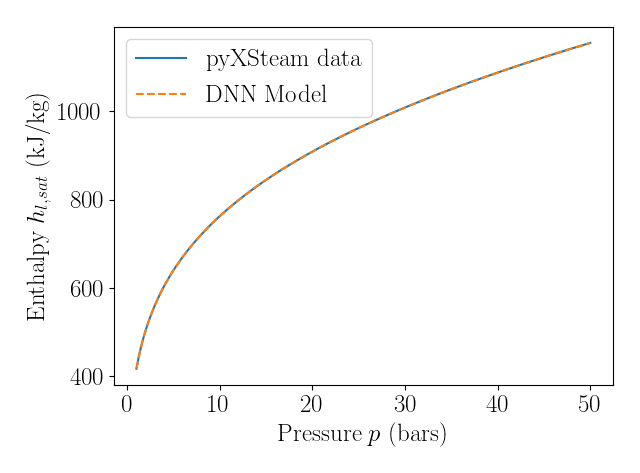
\includegraphics[width=0.5\linewidth]{Python/Models/DNN_Model_h_lsat.png}
    \resizebox{0.5\linewidth}{!}{%% Creator: Matplotlib, PGF backend
%%
%% To include the figure in your LaTeX document, write
%%   \input{<filename>.pgf}
%%
%% Make sure the required packages are loaded in your preamble
%%   \usepackage{pgf}
%%
%% Figures using additional raster images can only be included by \input if
%% they are in the same directory as the main LaTeX file. For loading figures
%% from other directories you can use the `import` package
%%   \usepackage{import}
%% and then include the figures with
%%   \import{<path to file>}{<filename>.pgf}
%%
%% Matplotlib used the following preamble
%%   \usepackage{fontspec}
%%   \setmainfont{DejaVuSerif.ttf}[Path=C:/Users/garaya/AppData/Local/Continuum/anaconda3/lib/site-packages/matplotlib/mpl-data/fonts/ttf/]
%%   \setsansfont{DejaVuSans.ttf}[Path=C:/Users/garaya/AppData/Local/Continuum/anaconda3/lib/site-packages/matplotlib/mpl-data/fonts/ttf/]
%%   \setmonofont{DejaVuSansMono.ttf}[Path=C:/Users/garaya/AppData/Local/Continuum/anaconda3/lib/site-packages/matplotlib/mpl-data/fonts/ttf/]
%%
\begingroup%
\makeatletter%
\begin{pgfpicture}%
\pgfpathrectangle{\pgfpointorigin}{\pgfqpoint{6.400000in}{4.730000in}}%
\pgfusepath{use as bounding box, clip}%
\begin{pgfscope}%
\pgfsetbuttcap%
\pgfsetmiterjoin%
\definecolor{currentfill}{rgb}{1.000000,1.000000,1.000000}%
\pgfsetfillcolor{currentfill}%
\pgfsetlinewidth{0.000000pt}%
\definecolor{currentstroke}{rgb}{1.000000,1.000000,1.000000}%
\pgfsetstrokecolor{currentstroke}%
\pgfsetdash{}{0pt}%
\pgfpathmoveto{\pgfqpoint{0.000000in}{0.000000in}}%
\pgfpathlineto{\pgfqpoint{6.400000in}{0.000000in}}%
\pgfpathlineto{\pgfqpoint{6.400000in}{4.730000in}}%
\pgfpathlineto{\pgfqpoint{0.000000in}{4.730000in}}%
\pgfpathclose%
\pgfusepath{fill}%
\end{pgfscope}%
\begin{pgfscope}%
\pgfsetbuttcap%
\pgfsetmiterjoin%
\definecolor{currentfill}{rgb}{1.000000,1.000000,1.000000}%
\pgfsetfillcolor{currentfill}%
\pgfsetlinewidth{0.000000pt}%
\definecolor{currentstroke}{rgb}{0.000000,0.000000,0.000000}%
\pgfsetstrokecolor{currentstroke}%
\pgfsetstrokeopacity{0.000000}%
\pgfsetdash{}{0pt}%
\pgfpathmoveto{\pgfqpoint{1.137518in}{0.879799in}}%
\pgfpathlineto{\pgfqpoint{6.130000in}{0.879799in}}%
\pgfpathlineto{\pgfqpoint{6.130000in}{4.463938in}}%
\pgfpathlineto{\pgfqpoint{1.137518in}{4.463938in}}%
\pgfpathclose%
\pgfusepath{fill}%
\end{pgfscope}%
\begin{pgfscope}%
\pgfsetbuttcap%
\pgfsetroundjoin%
\definecolor{currentfill}{rgb}{0.000000,0.000000,0.000000}%
\pgfsetfillcolor{currentfill}%
\pgfsetlinewidth{0.803000pt}%
\definecolor{currentstroke}{rgb}{0.000000,0.000000,0.000000}%
\pgfsetstrokecolor{currentstroke}%
\pgfsetdash{}{0pt}%
\pgfsys@defobject{currentmarker}{\pgfqpoint{0.000000in}{-0.048611in}}{\pgfqpoint{0.000000in}{0.000000in}}{%
\pgfpathmoveto{\pgfqpoint{0.000000in}{0.000000in}}%
\pgfpathlineto{\pgfqpoint{0.000000in}{-0.048611in}}%
\pgfusepath{stroke,fill}%
}%
\begin{pgfscope}%
\pgfsys@transformshift{1.271824in}{0.879799in}%
\pgfsys@useobject{currentmarker}{}%
\end{pgfscope}%
\end{pgfscope}%
\begin{pgfscope}%
\definecolor{textcolor}{rgb}{0.000000,0.000000,0.000000}%
\pgfsetstrokecolor{textcolor}%
\pgfsetfillcolor{textcolor}%
\pgftext[x=1.271824in,y=0.782577in,,top]{\color{textcolor}\rmfamily\fontsize{18.000000}{21.600000}\selectfont \(\displaystyle 0\)}%
\end{pgfscope}%
\begin{pgfscope}%
\pgfsetbuttcap%
\pgfsetroundjoin%
\definecolor{currentfill}{rgb}{0.000000,0.000000,0.000000}%
\pgfsetfillcolor{currentfill}%
\pgfsetlinewidth{0.803000pt}%
\definecolor{currentstroke}{rgb}{0.000000,0.000000,0.000000}%
\pgfsetstrokecolor{currentstroke}%
\pgfsetdash{}{0pt}%
\pgfsys@defobject{currentmarker}{\pgfqpoint{0.000000in}{-0.048611in}}{\pgfqpoint{0.000000in}{0.000000in}}{%
\pgfpathmoveto{\pgfqpoint{0.000000in}{0.000000in}}%
\pgfpathlineto{\pgfqpoint{0.000000in}{-0.048611in}}%
\pgfusepath{stroke,fill}%
}%
\begin{pgfscope}%
\pgfsys@transformshift{2.198073in}{0.879799in}%
\pgfsys@useobject{currentmarker}{}%
\end{pgfscope}%
\end{pgfscope}%
\begin{pgfscope}%
\definecolor{textcolor}{rgb}{0.000000,0.000000,0.000000}%
\pgfsetstrokecolor{textcolor}%
\pgfsetfillcolor{textcolor}%
\pgftext[x=2.198073in,y=0.782577in,,top]{\color{textcolor}\rmfamily\fontsize{18.000000}{21.600000}\selectfont \(\displaystyle 10\)}%
\end{pgfscope}%
\begin{pgfscope}%
\pgfsetbuttcap%
\pgfsetroundjoin%
\definecolor{currentfill}{rgb}{0.000000,0.000000,0.000000}%
\pgfsetfillcolor{currentfill}%
\pgfsetlinewidth{0.803000pt}%
\definecolor{currentstroke}{rgb}{0.000000,0.000000,0.000000}%
\pgfsetstrokecolor{currentstroke}%
\pgfsetdash{}{0pt}%
\pgfsys@defobject{currentmarker}{\pgfqpoint{0.000000in}{-0.048611in}}{\pgfqpoint{0.000000in}{0.000000in}}{%
\pgfpathmoveto{\pgfqpoint{0.000000in}{0.000000in}}%
\pgfpathlineto{\pgfqpoint{0.000000in}{-0.048611in}}%
\pgfusepath{stroke,fill}%
}%
\begin{pgfscope}%
\pgfsys@transformshift{3.124322in}{0.879799in}%
\pgfsys@useobject{currentmarker}{}%
\end{pgfscope}%
\end{pgfscope}%
\begin{pgfscope}%
\definecolor{textcolor}{rgb}{0.000000,0.000000,0.000000}%
\pgfsetstrokecolor{textcolor}%
\pgfsetfillcolor{textcolor}%
\pgftext[x=3.124322in,y=0.782577in,,top]{\color{textcolor}\rmfamily\fontsize{18.000000}{21.600000}\selectfont \(\displaystyle 20\)}%
\end{pgfscope}%
\begin{pgfscope}%
\pgfsetbuttcap%
\pgfsetroundjoin%
\definecolor{currentfill}{rgb}{0.000000,0.000000,0.000000}%
\pgfsetfillcolor{currentfill}%
\pgfsetlinewidth{0.803000pt}%
\definecolor{currentstroke}{rgb}{0.000000,0.000000,0.000000}%
\pgfsetstrokecolor{currentstroke}%
\pgfsetdash{}{0pt}%
\pgfsys@defobject{currentmarker}{\pgfqpoint{0.000000in}{-0.048611in}}{\pgfqpoint{0.000000in}{0.000000in}}{%
\pgfpathmoveto{\pgfqpoint{0.000000in}{0.000000in}}%
\pgfpathlineto{\pgfqpoint{0.000000in}{-0.048611in}}%
\pgfusepath{stroke,fill}%
}%
\begin{pgfscope}%
\pgfsys@transformshift{4.050571in}{0.879799in}%
\pgfsys@useobject{currentmarker}{}%
\end{pgfscope}%
\end{pgfscope}%
\begin{pgfscope}%
\definecolor{textcolor}{rgb}{0.000000,0.000000,0.000000}%
\pgfsetstrokecolor{textcolor}%
\pgfsetfillcolor{textcolor}%
\pgftext[x=4.050571in,y=0.782577in,,top]{\color{textcolor}\rmfamily\fontsize{18.000000}{21.600000}\selectfont \(\displaystyle 30\)}%
\end{pgfscope}%
\begin{pgfscope}%
\pgfsetbuttcap%
\pgfsetroundjoin%
\definecolor{currentfill}{rgb}{0.000000,0.000000,0.000000}%
\pgfsetfillcolor{currentfill}%
\pgfsetlinewidth{0.803000pt}%
\definecolor{currentstroke}{rgb}{0.000000,0.000000,0.000000}%
\pgfsetstrokecolor{currentstroke}%
\pgfsetdash{}{0pt}%
\pgfsys@defobject{currentmarker}{\pgfqpoint{0.000000in}{-0.048611in}}{\pgfqpoint{0.000000in}{0.000000in}}{%
\pgfpathmoveto{\pgfqpoint{0.000000in}{0.000000in}}%
\pgfpathlineto{\pgfqpoint{0.000000in}{-0.048611in}}%
\pgfusepath{stroke,fill}%
}%
\begin{pgfscope}%
\pgfsys@transformshift{4.976820in}{0.879799in}%
\pgfsys@useobject{currentmarker}{}%
\end{pgfscope}%
\end{pgfscope}%
\begin{pgfscope}%
\definecolor{textcolor}{rgb}{0.000000,0.000000,0.000000}%
\pgfsetstrokecolor{textcolor}%
\pgfsetfillcolor{textcolor}%
\pgftext[x=4.976820in,y=0.782577in,,top]{\color{textcolor}\rmfamily\fontsize{18.000000}{21.600000}\selectfont \(\displaystyle 40\)}%
\end{pgfscope}%
\begin{pgfscope}%
\pgfsetbuttcap%
\pgfsetroundjoin%
\definecolor{currentfill}{rgb}{0.000000,0.000000,0.000000}%
\pgfsetfillcolor{currentfill}%
\pgfsetlinewidth{0.803000pt}%
\definecolor{currentstroke}{rgb}{0.000000,0.000000,0.000000}%
\pgfsetstrokecolor{currentstroke}%
\pgfsetdash{}{0pt}%
\pgfsys@defobject{currentmarker}{\pgfqpoint{0.000000in}{-0.048611in}}{\pgfqpoint{0.000000in}{0.000000in}}{%
\pgfpathmoveto{\pgfqpoint{0.000000in}{0.000000in}}%
\pgfpathlineto{\pgfqpoint{0.000000in}{-0.048611in}}%
\pgfusepath{stroke,fill}%
}%
\begin{pgfscope}%
\pgfsys@transformshift{5.903069in}{0.879799in}%
\pgfsys@useobject{currentmarker}{}%
\end{pgfscope}%
\end{pgfscope}%
\begin{pgfscope}%
\definecolor{textcolor}{rgb}{0.000000,0.000000,0.000000}%
\pgfsetstrokecolor{textcolor}%
\pgfsetfillcolor{textcolor}%
\pgftext[x=5.903069in,y=0.782577in,,top]{\color{textcolor}\rmfamily\fontsize{18.000000}{21.600000}\selectfont \(\displaystyle 50\)}%
\end{pgfscope}%
\begin{pgfscope}%
\definecolor{textcolor}{rgb}{0.000000,0.000000,0.000000}%
\pgfsetstrokecolor{textcolor}%
\pgfsetfillcolor{textcolor}%
\pgftext[x=3.633759in,y=0.485078in,,top]{\color{textcolor}\rmfamily\fontsize{18.000000}{21.600000}\selectfont Pressure \(\displaystyle p\) (bars)}%
\end{pgfscope}%
\begin{pgfscope}%
\pgfsetbuttcap%
\pgfsetroundjoin%
\definecolor{currentfill}{rgb}{0.000000,0.000000,0.000000}%
\pgfsetfillcolor{currentfill}%
\pgfsetlinewidth{0.803000pt}%
\definecolor{currentstroke}{rgb}{0.000000,0.000000,0.000000}%
\pgfsetstrokecolor{currentstroke}%
\pgfsetdash{}{0pt}%
\pgfsys@defobject{currentmarker}{\pgfqpoint{-0.048611in}{0.000000in}}{\pgfqpoint{0.000000in}{0.000000in}}{%
\pgfpathmoveto{\pgfqpoint{0.000000in}{0.000000in}}%
\pgfpathlineto{\pgfqpoint{-0.048611in}{0.000000in}}%
\pgfusepath{stroke,fill}%
}%
\begin{pgfscope}%
\pgfsys@transformshift{1.137518in}{0.965634in}%
\pgfsys@useobject{currentmarker}{}%
\end{pgfscope}%
\end{pgfscope}%
\begin{pgfscope}%
\definecolor{textcolor}{rgb}{0.000000,0.000000,0.000000}%
\pgfsetstrokecolor{textcolor}%
\pgfsetfillcolor{textcolor}%
\pgftext[x=0.710091in,y=0.870663in,left,base]{\color{textcolor}\rmfamily\fontsize{18.000000}{21.600000}\selectfont \(\displaystyle 400\)}%
\end{pgfscope}%
\begin{pgfscope}%
\pgfsetbuttcap%
\pgfsetroundjoin%
\definecolor{currentfill}{rgb}{0.000000,0.000000,0.000000}%
\pgfsetfillcolor{currentfill}%
\pgfsetlinewidth{0.803000pt}%
\definecolor{currentstroke}{rgb}{0.000000,0.000000,0.000000}%
\pgfsetstrokecolor{currentstroke}%
\pgfsetdash{}{0pt}%
\pgfsys@defobject{currentmarker}{\pgfqpoint{-0.048611in}{0.000000in}}{\pgfqpoint{0.000000in}{0.000000in}}{%
\pgfpathmoveto{\pgfqpoint{0.000000in}{0.000000in}}%
\pgfpathlineto{\pgfqpoint{-0.048611in}{0.000000in}}%
\pgfusepath{stroke,fill}%
}%
\begin{pgfscope}%
\pgfsys@transformshift{1.137518in}{1.849763in}%
\pgfsys@useobject{currentmarker}{}%
\end{pgfscope}%
\end{pgfscope}%
\begin{pgfscope}%
\definecolor{textcolor}{rgb}{0.000000,0.000000,0.000000}%
\pgfsetstrokecolor{textcolor}%
\pgfsetfillcolor{textcolor}%
\pgftext[x=0.710091in,y=1.754793in,left,base]{\color{textcolor}\rmfamily\fontsize{18.000000}{21.600000}\selectfont \(\displaystyle 600\)}%
\end{pgfscope}%
\begin{pgfscope}%
\pgfsetbuttcap%
\pgfsetroundjoin%
\definecolor{currentfill}{rgb}{0.000000,0.000000,0.000000}%
\pgfsetfillcolor{currentfill}%
\pgfsetlinewidth{0.803000pt}%
\definecolor{currentstroke}{rgb}{0.000000,0.000000,0.000000}%
\pgfsetstrokecolor{currentstroke}%
\pgfsetdash{}{0pt}%
\pgfsys@defobject{currentmarker}{\pgfqpoint{-0.048611in}{0.000000in}}{\pgfqpoint{0.000000in}{0.000000in}}{%
\pgfpathmoveto{\pgfqpoint{0.000000in}{0.000000in}}%
\pgfpathlineto{\pgfqpoint{-0.048611in}{0.000000in}}%
\pgfusepath{stroke,fill}%
}%
\begin{pgfscope}%
\pgfsys@transformshift{1.137518in}{2.733893in}%
\pgfsys@useobject{currentmarker}{}%
\end{pgfscope}%
\end{pgfscope}%
\begin{pgfscope}%
\definecolor{textcolor}{rgb}{0.000000,0.000000,0.000000}%
\pgfsetstrokecolor{textcolor}%
\pgfsetfillcolor{textcolor}%
\pgftext[x=0.710091in,y=2.638922in,left,base]{\color{textcolor}\rmfamily\fontsize{18.000000}{21.600000}\selectfont \(\displaystyle 800\)}%
\end{pgfscope}%
\begin{pgfscope}%
\pgfsetbuttcap%
\pgfsetroundjoin%
\definecolor{currentfill}{rgb}{0.000000,0.000000,0.000000}%
\pgfsetfillcolor{currentfill}%
\pgfsetlinewidth{0.803000pt}%
\definecolor{currentstroke}{rgb}{0.000000,0.000000,0.000000}%
\pgfsetstrokecolor{currentstroke}%
\pgfsetdash{}{0pt}%
\pgfsys@defobject{currentmarker}{\pgfqpoint{-0.048611in}{0.000000in}}{\pgfqpoint{0.000000in}{0.000000in}}{%
\pgfpathmoveto{\pgfqpoint{0.000000in}{0.000000in}}%
\pgfpathlineto{\pgfqpoint{-0.048611in}{0.000000in}}%
\pgfusepath{stroke,fill}%
}%
\begin{pgfscope}%
\pgfsys@transformshift{1.137518in}{3.618023in}%
\pgfsys@useobject{currentmarker}{}%
\end{pgfscope}%
\end{pgfscope}%
\begin{pgfscope}%
\definecolor{textcolor}{rgb}{0.000000,0.000000,0.000000}%
\pgfsetstrokecolor{textcolor}%
\pgfsetfillcolor{textcolor}%
\pgftext[x=0.600023in,y=3.523052in,left,base]{\color{textcolor}\rmfamily\fontsize{18.000000}{21.600000}\selectfont \(\displaystyle 1000\)}%
\end{pgfscope}%
\begin{pgfscope}%
\definecolor{textcolor}{rgb}{0.000000,0.000000,0.000000}%
\pgfsetstrokecolor{textcolor}%
\pgfsetfillcolor{textcolor}%
\pgftext[x=0.544467in,y=2.671868in,,bottom,rotate=90.000000]{\color{textcolor}\rmfamily\fontsize{18.000000}{21.600000}\selectfont Enthalpy \(\displaystyle h_{l,sat}\) (kJ/kg)}%
\end{pgfscope}%
\begin{pgfscope}%
\pgfpathrectangle{\pgfqpoint{1.137518in}{0.879799in}}{\pgfqpoint{4.992482in}{3.584139in}}%
\pgfusepath{clip}%
\pgfsetrectcap%
\pgfsetroundjoin%
\pgfsetlinewidth{1.505625pt}%
\definecolor{currentstroke}{rgb}{0.121569,0.466667,0.705882}%
\pgfsetstrokecolor{currentstroke}%
\pgfsetdash{}{0pt}%
\pgfpathmoveto{\pgfqpoint{1.364449in}{1.042714in}}%
\pgfpathlineto{\pgfqpoint{1.387199in}{1.159540in}}%
\pgfpathlineto{\pgfqpoint{1.409949in}{1.258879in}}%
\pgfpathlineto{\pgfqpoint{1.432699in}{1.345730in}}%
\pgfpathlineto{\pgfqpoint{1.455449in}{1.423174in}}%
\pgfpathlineto{\pgfqpoint{1.478199in}{1.493255in}}%
\pgfpathlineto{\pgfqpoint{1.500949in}{1.557402in}}%
\pgfpathlineto{\pgfqpoint{1.523699in}{1.616654in}}%
\pgfpathlineto{\pgfqpoint{1.557823in}{1.698014in}}%
\pgfpathlineto{\pgfqpoint{1.591948in}{1.772020in}}%
\pgfpathlineto{\pgfqpoint{1.626073in}{1.840047in}}%
\pgfpathlineto{\pgfqpoint{1.660198in}{1.903110in}}%
\pgfpathlineto{\pgfqpoint{1.694323in}{1.961977in}}%
\pgfpathlineto{\pgfqpoint{1.728448in}{2.017248in}}%
\pgfpathlineto{\pgfqpoint{1.773948in}{2.086156in}}%
\pgfpathlineto{\pgfqpoint{1.819448in}{2.150391in}}%
\pgfpathlineto{\pgfqpoint{1.864948in}{2.210637in}}%
\pgfpathlineto{\pgfqpoint{1.910448in}{2.267434in}}%
\pgfpathlineto{\pgfqpoint{1.955948in}{2.321217in}}%
\pgfpathlineto{\pgfqpoint{2.012823in}{2.384741in}}%
\pgfpathlineto{\pgfqpoint{2.069698in}{2.444666in}}%
\pgfpathlineto{\pgfqpoint{2.126573in}{2.501446in}}%
\pgfpathlineto{\pgfqpoint{2.183448in}{2.555450in}}%
\pgfpathlineto{\pgfqpoint{2.251698in}{2.617019in}}%
\pgfpathlineto{\pgfqpoint{2.319948in}{2.675466in}}%
\pgfpathlineto{\pgfqpoint{2.388198in}{2.731150in}}%
\pgfpathlineto{\pgfqpoint{2.467823in}{2.793018in}}%
\pgfpathlineto{\pgfqpoint{2.547447in}{2.851923in}}%
\pgfpathlineto{\pgfqpoint{2.627072in}{2.908193in}}%
\pgfpathlineto{\pgfqpoint{2.718072in}{2.969622in}}%
\pgfpathlineto{\pgfqpoint{2.809072in}{3.028308in}}%
\pgfpathlineto{\pgfqpoint{2.900072in}{3.084536in}}%
\pgfpathlineto{\pgfqpoint{3.002447in}{3.145157in}}%
\pgfpathlineto{\pgfqpoint{3.104822in}{3.203267in}}%
\pgfpathlineto{\pgfqpoint{3.218572in}{3.265190in}}%
\pgfpathlineto{\pgfqpoint{3.332322in}{3.324607in}}%
\pgfpathlineto{\pgfqpoint{3.457447in}{3.387364in}}%
\pgfpathlineto{\pgfqpoint{3.582571in}{3.447661in}}%
\pgfpathlineto{\pgfqpoint{3.719071in}{3.510912in}}%
\pgfpathlineto{\pgfqpoint{3.855571in}{3.571778in}}%
\pgfpathlineto{\pgfqpoint{4.003446in}{3.635284in}}%
\pgfpathlineto{\pgfqpoint{4.162696in}{3.701117in}}%
\pgfpathlineto{\pgfqpoint{4.321946in}{3.764551in}}%
\pgfpathlineto{\pgfqpoint{4.492570in}{3.830107in}}%
\pgfpathlineto{\pgfqpoint{4.674570in}{3.897546in}}%
\pgfpathlineto{\pgfqpoint{4.856570in}{3.962656in}}%
\pgfpathlineto{\pgfqpoint{5.049945in}{4.029522in}}%
\pgfpathlineto{\pgfqpoint{5.254695in}{4.097960in}}%
\pgfpathlineto{\pgfqpoint{5.470819in}{4.167811in}}%
\pgfpathlineto{\pgfqpoint{5.698319in}{4.238933in}}%
\pgfpathlineto{\pgfqpoint{5.903069in}{4.301022in}}%
\pgfpathlineto{\pgfqpoint{5.903069in}{4.301022in}}%
\pgfusepath{stroke}%
\end{pgfscope}%
\begin{pgfscope}%
\pgfpathrectangle{\pgfqpoint{1.137518in}{0.879799in}}{\pgfqpoint{4.992482in}{3.584139in}}%
\pgfusepath{clip}%
\pgfsetbuttcap%
\pgfsetroundjoin%
\pgfsetlinewidth{1.505625pt}%
\definecolor{currentstroke}{rgb}{1.000000,0.498039,0.054902}%
\pgfsetstrokecolor{currentstroke}%
\pgfsetdash{{5.550000pt}{2.400000pt}}{0.000000pt}%
\pgfpathmoveto{\pgfqpoint{1.364449in}{1.042759in}}%
\pgfpathlineto{\pgfqpoint{1.387199in}{1.159466in}}%
\pgfpathlineto{\pgfqpoint{1.409949in}{1.258951in}}%
\pgfpathlineto{\pgfqpoint{1.432699in}{1.345792in}}%
\pgfpathlineto{\pgfqpoint{1.455449in}{1.423092in}}%
\pgfpathlineto{\pgfqpoint{1.478199in}{1.493138in}}%
\pgfpathlineto{\pgfqpoint{1.500949in}{1.557392in}}%
\pgfpathlineto{\pgfqpoint{1.523699in}{1.616767in}}%
\pgfpathlineto{\pgfqpoint{1.557823in}{1.698132in}}%
\pgfpathlineto{\pgfqpoint{1.591948in}{1.771969in}}%
\pgfpathlineto{\pgfqpoint{1.626073in}{1.839878in}}%
\pgfpathlineto{\pgfqpoint{1.660198in}{1.902987in}}%
\pgfpathlineto{\pgfqpoint{1.694323in}{1.962008in}}%
\pgfpathlineto{\pgfqpoint{1.728448in}{2.017412in}}%
\pgfpathlineto{\pgfqpoint{1.773948in}{2.086331in}}%
\pgfpathlineto{\pgfqpoint{1.819448in}{2.150405in}}%
\pgfpathlineto{\pgfqpoint{1.864948in}{2.210473in}}%
\pgfpathlineto{\pgfqpoint{1.910448in}{2.267206in}}%
\pgfpathlineto{\pgfqpoint{1.967323in}{2.334127in}}%
\pgfpathlineto{\pgfqpoint{2.024198in}{2.397105in}}%
\pgfpathlineto{\pgfqpoint{2.081073in}{2.456506in}}%
\pgfpathlineto{\pgfqpoint{2.137948in}{2.512678in}}%
\pgfpathlineto{\pgfqpoint{2.194823in}{2.566006in}}%
\pgfpathlineto{\pgfqpoint{2.263073in}{2.626796in}}%
\pgfpathlineto{\pgfqpoint{2.331323in}{2.684641in}}%
\pgfpathlineto{\pgfqpoint{2.410948in}{2.748941in}}%
\pgfpathlineto{\pgfqpoint{2.490573in}{2.810159in}}%
\pgfpathlineto{\pgfqpoint{2.570197in}{2.868498in}}%
\pgfpathlineto{\pgfqpoint{2.649822in}{2.924141in}}%
\pgfpathlineto{\pgfqpoint{2.729447in}{2.977319in}}%
\pgfpathlineto{\pgfqpoint{2.820447in}{3.035442in}}%
\pgfpathlineto{\pgfqpoint{2.922822in}{3.097964in}}%
\pgfpathlineto{\pgfqpoint{3.025197in}{3.157929in}}%
\pgfpathlineto{\pgfqpoint{3.138947in}{3.221930in}}%
\pgfpathlineto{\pgfqpoint{3.252697in}{3.283354in}}%
\pgfpathlineto{\pgfqpoint{3.366447in}{3.342292in}}%
\pgfpathlineto{\pgfqpoint{3.480196in}{3.398858in}}%
\pgfpathlineto{\pgfqpoint{3.605321in}{3.458572in}}%
\pgfpathlineto{\pgfqpoint{3.741821in}{3.521109in}}%
\pgfpathlineto{\pgfqpoint{3.889696in}{3.586300in}}%
\pgfpathlineto{\pgfqpoint{4.048946in}{3.654009in}}%
\pgfpathlineto{\pgfqpoint{4.208196in}{3.719388in}}%
\pgfpathlineto{\pgfqpoint{4.367446in}{3.782491in}}%
\pgfpathlineto{\pgfqpoint{4.526695in}{3.843315in}}%
\pgfpathlineto{\pgfqpoint{4.697320in}{3.906058in}}%
\pgfpathlineto{\pgfqpoint{4.879320in}{3.970542in}}%
\pgfpathlineto{\pgfqpoint{5.084070in}{4.040694in}}%
\pgfpathlineto{\pgfqpoint{5.322945in}{4.120117in}}%
\pgfpathlineto{\pgfqpoint{5.550444in}{4.193407in}}%
\pgfpathlineto{\pgfqpoint{5.732444in}{4.249720in}}%
\pgfpathlineto{\pgfqpoint{5.880319in}{4.293254in}}%
\pgfpathlineto{\pgfqpoint{5.903069in}{4.299734in}}%
\pgfpathlineto{\pgfqpoint{5.903069in}{4.299734in}}%
\pgfusepath{stroke}%
\end{pgfscope}%
\begin{pgfscope}%
\pgfsetrectcap%
\pgfsetmiterjoin%
\pgfsetlinewidth{0.803000pt}%
\definecolor{currentstroke}{rgb}{0.000000,0.000000,0.000000}%
\pgfsetstrokecolor{currentstroke}%
\pgfsetdash{}{0pt}%
\pgfpathmoveto{\pgfqpoint{1.137518in}{0.879799in}}%
\pgfpathlineto{\pgfqpoint{1.137518in}{4.463938in}}%
\pgfusepath{stroke}%
\end{pgfscope}%
\begin{pgfscope}%
\pgfsetrectcap%
\pgfsetmiterjoin%
\pgfsetlinewidth{0.803000pt}%
\definecolor{currentstroke}{rgb}{0.000000,0.000000,0.000000}%
\pgfsetstrokecolor{currentstroke}%
\pgfsetdash{}{0pt}%
\pgfpathmoveto{\pgfqpoint{6.130000in}{0.879799in}}%
\pgfpathlineto{\pgfqpoint{6.130000in}{4.463938in}}%
\pgfusepath{stroke}%
\end{pgfscope}%
\begin{pgfscope}%
\pgfsetrectcap%
\pgfsetmiterjoin%
\pgfsetlinewidth{0.803000pt}%
\definecolor{currentstroke}{rgb}{0.000000,0.000000,0.000000}%
\pgfsetstrokecolor{currentstroke}%
\pgfsetdash{}{0pt}%
\pgfpathmoveto{\pgfqpoint{1.137518in}{0.879799in}}%
\pgfpathlineto{\pgfqpoint{6.130000in}{0.879799in}}%
\pgfusepath{stroke}%
\end{pgfscope}%
\begin{pgfscope}%
\pgfsetrectcap%
\pgfsetmiterjoin%
\pgfsetlinewidth{0.803000pt}%
\definecolor{currentstroke}{rgb}{0.000000,0.000000,0.000000}%
\pgfsetstrokecolor{currentstroke}%
\pgfsetdash{}{0pt}%
\pgfpathmoveto{\pgfqpoint{1.137518in}{4.463938in}}%
\pgfpathlineto{\pgfqpoint{6.130000in}{4.463938in}}%
\pgfusepath{stroke}%
\end{pgfscope}%
\begin{pgfscope}%
\pgfsetbuttcap%
\pgfsetmiterjoin%
\definecolor{currentfill}{rgb}{1.000000,1.000000,1.000000}%
\pgfsetfillcolor{currentfill}%
\pgfsetfillopacity{0.800000}%
\pgfsetlinewidth{1.003750pt}%
\definecolor{currentstroke}{rgb}{0.800000,0.800000,0.800000}%
\pgfsetstrokecolor{currentstroke}%
\pgfsetstrokeopacity{0.800000}%
\pgfsetdash{}{0pt}%
\pgfpathmoveto{\pgfqpoint{3.231904in}{1.004799in}}%
\pgfpathlineto{\pgfqpoint{5.955000in}{1.004799in}}%
\pgfpathquadraticcurveto{\pgfqpoint{6.005000in}{1.004799in}}{\pgfqpoint{6.005000in}{1.054799in}}%
\pgfpathlineto{\pgfqpoint{6.005000in}{1.767225in}}%
\pgfpathquadraticcurveto{\pgfqpoint{6.005000in}{1.817225in}}{\pgfqpoint{5.955000in}{1.817225in}}%
\pgfpathlineto{\pgfqpoint{3.231904in}{1.817225in}}%
\pgfpathquadraticcurveto{\pgfqpoint{3.181904in}{1.817225in}}{\pgfqpoint{3.181904in}{1.767225in}}%
\pgfpathlineto{\pgfqpoint{3.181904in}{1.054799in}}%
\pgfpathquadraticcurveto{\pgfqpoint{3.181904in}{1.004799in}}{\pgfqpoint{3.231904in}{1.004799in}}%
\pgfpathclose%
\pgfusepath{stroke,fill}%
\end{pgfscope}%
\begin{pgfscope}%
\pgfsetrectcap%
\pgfsetroundjoin%
\pgfsetlinewidth{1.505625pt}%
\definecolor{currentstroke}{rgb}{0.121569,0.466667,0.705882}%
\pgfsetstrokecolor{currentstroke}%
\pgfsetdash{}{0pt}%
\pgfpathmoveto{\pgfqpoint{3.281904in}{1.614784in}}%
\pgfpathlineto{\pgfqpoint{3.781904in}{1.614784in}}%
\pgfusepath{stroke}%
\end{pgfscope}%
\begin{pgfscope}%
\definecolor{textcolor}{rgb}{0.000000,0.000000,0.000000}%
\pgfsetstrokecolor{textcolor}%
\pgfsetfillcolor{textcolor}%
\pgftext[x=3.981904in,y=1.527284in,left,base]{\color{textcolor}\rmfamily\fontsize{18.000000}{21.600000}\selectfont pyXSteam data}%
\end{pgfscope}%
\begin{pgfscope}%
\pgfsetbuttcap%
\pgfsetroundjoin%
\pgfsetlinewidth{1.505625pt}%
\definecolor{currentstroke}{rgb}{1.000000,0.498039,0.054902}%
\pgfsetstrokecolor{currentstroke}%
\pgfsetdash{{5.550000pt}{2.400000pt}}{0.000000pt}%
\pgfpathmoveto{\pgfqpoint{3.281904in}{1.244301in}}%
\pgfpathlineto{\pgfqpoint{3.781904in}{1.244301in}}%
\pgfusepath{stroke}%
\end{pgfscope}%
\begin{pgfscope}%
\definecolor{textcolor}{rgb}{0.000000,0.000000,0.000000}%
\pgfsetstrokecolor{textcolor}%
\pgfsetfillcolor{textcolor}%
\pgftext[x=3.981904in,y=1.156801in,left,base]{\color{textcolor}\rmfamily\fontsize{18.000000}{21.600000}\selectfont DNN Model}%
\end{pgfscope}%
\end{pgfpicture}%
\makeatother%
\endgroup%
}
    \caption{Entraînement d'un réseau de neurones annexe pour l'enthalpie massique du liquide à saturation à partir de données issues de pyXSteam. Le \textit{root mean square} (RMS) de l'écart relatif vaut $ \text{RMS}\left(\frac{h_{DNN}-h_{XSteam}}{h_{XSteam}}\right)  = \num{6.29e-5}$.}
    \label{fig:DNN_enthalpy}
\end{figure}

Ainsi, pour l'équation d'énergie, on est capable de construire un graphe d'opérations dérivables 
\begin{equation}
    H : z \rightarrow h_{l,sat}(p(z)) + x(z)h_{vl,sat}(p(z))
\end{equation}
Avec $\pder[H]{z}$ obtenu en un bloc. Concrètement, on utilise \verb|tf.gradients(H,z)| avec Tensorflow qui sera évalué pour tous les points de $V^{\text{int}}$. Ainsi :

\begin{equation}
    \mathcal{L}_{\text{Energie}} =\frac{1}{N^{\text{int}}}\sum_{z\in V^{\text{int}}} \left( \frac{DG}{4q''}\pder{z}\left[ h_{l,sat}(p(z)) + x(z)h_{vl,sat}(p(z)) \right] -1  \right)^2
    \label{eq:titrednn}
\end{equation}

La même structure d'erreur est constituée pour les deux autres équations. A ce titre, il faut aborder le point de la \textbf{normalisation}. En effet, on travaille avec des grandeurs dimensionnées qui peuvent être d'un ordre de grandeur très différent : $x$ varie usuellement entre $0$ et $1$ et donc on s'attend à ce que $\mathcal{L}_{\text{Drift Flux Model}}\sim 1$. En revanche, $4q''/DG \sim 10^2$ donc $\mathcal{L}_{\text{Energie}}$ peut être de l'ordre de $10^4$ si on l'implémente comme dans l'équation \ref{eq:titre}. Cela explique pourquoi l'équation \ref{eq:titrednn} a un $-1$ comme terme de droite. En effet, il est difficile d'optimiser simultanément une somme de plusieurs termes qui sont d'ordre de grandeurs très différents. Une solution plus simple aurait été de travailler dès le début avec des grandeurs adimensionnés. Cela ne s'est pas fait car il y a beaucoup de relations thermodynamiques et de coefficients dimensionnés définis implicitement.\\

Enfin, la question de l'initialisation des réseaux de neurones pour la résolution de $\epsilon, x$ et $p$ est un sujet compliqué dont on ne traitera pas en profondeur dans ce rapport. En pratique, après une initialisation aléatoire, on effectue une pré-optimisation vers un set de fonctions affines afin de gommer l'"indéterminisme".\\


A travers cette section nous avons tenté d'introduire le formalisme PINN et quelques détails qui nous semblaient importants. Comme vous le constaterez par les dates des articles (la plupart n'étant pas paru avant 2019), le sujet est tout récent et manque donc encore de maturité. Nous n'avons pas non plus cherché à être exhaustif car ce n'est pas l'objet de ce rapport. De même la bibliographie a été réduite à quelques exemples pertinents et est loin d'être complète. L'idée a été motivée par un projet de maîtrise portant sur les PINNs dans un domaine connexe. Si vous avez des questions ou souhaitez en savoir davantage, n'hésitez pas à nous contacter.

\subsection{Limites rencontrées}

Dans le cadre du projet, nous avons rencontré plusieurs difficultés à adapter la méthode PINN pour des raisons parfois spécifiques à la nature du problème. En particulier les modèles de corrélation complexes avec des seuils, des conditions posent des soucis de différentiation. De même il faut bien veiller à n'appliquer les équations du modèle diphasique lorsque $0<x<1$ et veiller à ce que l'on retombe sur des équations monophasiques aux bords ce qui créé d'autres sources d'instabilités avec des gradients infinis. Enfin nous avons tenté de supprimer toute les possibilités d'obtenir un numérateur nul en écrivant les équations de la manière la plus adéquat. Il demeure quelques sources de problèmes tout de même. En particulier nous n'avons pas pu résoudre correctement le problème du sueil $x=0$ dans le modèle de corrélation (où on pénalise l'écart à $\varepsilon = 0$ quand $x<0$).\\

De manière plus générale, le choix des fonctions d'activation et de la taille des réseaux est encore assez empirique et sujet à discussion. Ceci dit, il reste un grand nombre de possibilités à explorer tant dans les détails que dans la méthode. L'une d'entre elle serait d'établir des modèles de corrélation directement avec des réseaux de neurones en utilisant des données expérimentales dans davantage de cas.

